\documentclass[conference]{IEEEtran}
\usepackage{cite,amsmath,amssymb,graphicx,booktabs,array,url,textcomp}
\hyphenation{XGBoost}
\begin{document}
\title{Predicting a Water Quality Index Without Data Leakage: A Study Using Classical Machine Learning}
\author{\IEEEauthorblockN{T109: Priyal, Anusha, Sarthak, Kashika and Vaishnavi}
\IEEEauthorblockA{Newton School of Technology\\
Advanced Machine Learning / Deep Learning, Project 18\\
Code: \url{https://github.com/Priyal-2005/water-quality-prediction}}}
\maketitle
\begin{abstract}
A water quality index turns several water measurements into one score between 0 and 100. We train models to predict this score (the CCME index) from a small set of readings and compare four models: a baseline that always guesses the average, Ridge Regression, Random Forest and XGBoost. The index is calculated from eight measurements, so giving all eight to a model lets it simply work out the formula (R$^2$ = 0.991). We therefore hide five of them, and test on monitoring stations the models have never seen and, separately, on later years. On unseen stations XGBoost was best (MAE 7.543, RMSE 11.058, R$^2$ = 0.293), slightly ahead of Random Forest (R$^2$ = 0.278); on later years it reached R$^2$ = 0.243. The models predict polluted water to be better than it is, and much of their skill comes from knowing the country and the past readings of a station.
\end{abstract}
\begin{IEEEkeywords}
water quality index, regression, Random Forest, XGBoost, data leakage, SHAP
\end{IEEEkeywords}
\section{Introduction}
Authorities test rivers, lakes and coastal water to protect people and nature. A water quality index combines many measurements into one number that is easy to report and compare. A model that predicts this number from a few simple readings could help with screening, but only if the test is fair. If the model is given the same measurements the index is calculated from, it can just recompute the formula.

In this project we predict \texttt{target\_ccme\_value}, a CCME water quality index between 0 and 100 (higher means cleaner water). Our main contributions are:

\begin{itemize}
\item an experiment that shows how much the formula leaks when all measurements are given, and a smaller input set that avoids it;
\item a fair test on stations the models have never seen, plus a second test on later years;
\item a comparison of four models using MAE, RMSE and R$^2$, with confidence intervals and a look at where the models go wrong.
\end{itemize}

The report reviews related work, describes the data and methods, and then gives the results, limitations and our plan for Phase 2. The code, data and results are in our GitHub repository: \url{https://github.com/Priyal-2005/water-quality-prediction}.


\section{Related work}
The CCME index is based on how many measurements break their guideline, how often, and by how much~\cite{ccme2001}. Reviews describe many water quality indices and their weaknesses: one very bad measurement can be hidden by good ones, and the choice of measurements is partly subjective~\cite{syeed2023,chidiac2023}. Karim et al. released a large dataset of surface-water measurements from 1940 to 2023~\cite{karim2025}. We use only a cleaned part of it.

Random Forests use many decision trees built on random parts of the data~\cite{breiman2001}. Gradient boosting builds a model step by step, where each step fixes the mistakes of the earlier ones~\cite{friedman2001}, and XGBoost is a fast version of this idea~\cite{chen2016}. SHAP shows how much each input pushed a prediction up or down~\cite{lundberg2017}; it shows what the model uses, not what causes pollution. Other studies found that deep neural networks do not always beat tree models on table-like data~\cite{grinsztajn2022,shwartz2022}.

Studies use different tasks and measures, so their results are hard to compare. Ooko et al. found that Random Forest worked best, with 79\% accuracy, in a classification study~\cite{ooko2023}. Rahman et al. reported 97.33\% accuracy for five CCME classes on the Canadian part of the same dataset, using the eight measurements as inputs~\cite{rahman2026}. Since the index is calculated from those eight, such scores cannot be compared with ours (Section~\ref{sec:leak}).

The gap we focus on is how models are tested. Scores look better than they are when the model sees the measurements the target is made from, or when the same station is in both training and test data. We hide five main measurements, test on unseen stations and later years, and use the same measures for every model.


\section{Dataset and target}
After cleaning, our dataset has \textbf{259,774 rows} from \textbf{9,940 monitoring stations} in England, Ireland, the USA and Canada, from 2000 to 2023. The target is the CCME score, and 43.7\% of the rows are exactly 100. The original dataset has 2.82 million records from five countries~\cite{karim2025}; we keep a part of it that suits our fair-testing plan.

We removed effluent, sewage and drainage samples (not surface water), records before 2000, exact duplicates and impossible values. The authors of the source data had also filled many gaps with one repeated number per country and water type (for example, dissolved oxygen 10.2 in 360,401 rows from England). Real measurements do not repeat like this, so we found these values by how often they appeared and marked them as missing. They may still affect the score, because the index was calculated after the gaps were filled. Finally, we kept whole stations when reducing the size of the dataset.

\begin{table}[!t]\caption{Rows removed at each cleaning step.}\centering
{\footnotesize\setlength{\tabcolsep}{3pt}\begin{tabular}{>{\raggedright\arraybackslash}p{0.62\linewidth}r}\toprule
\textbf{Cleaning step} & \textbf{Rows}\\\midrule
Effluent, sewage, drainage removed & 635,532\\
Records before 2000 removed & 243,089\\
Exact duplicates removed & 7,277\\
Rows with fewer than 5 of 8 real measurements removed & 474,227\\
Whole stations sampled to keep the dataset small & 1,162,081\\
Final dataset after keeping whole stations & 259,774\\
\bottomrule\end{tabular}}
\end{table}

\subsection{EDA on the raw data and its basic issues}
Before cleaning we looked at the raw file: 2,781,980 rows. It is very uneven: England has 76.5\% of the rows, the USA 14.9\%, Ireland 8.5\% and Canada only 0.1\%. All sewage, effluent and drainage rows are from England (29.9\% of its raw rows).

The basic problems in the raw data were: (1) sewage, effluent and drainage samples; (2) records before 2000; (3) duplicates; (4) rows with too few real measurements; (5) England dominating the data; and (6) gaps filled with repeated numbers.

The biggest surprise was the filler numbers. A histogram of a real measurement is smooth, but in the raw England river data dissolved oxygen, pH and temperature each have one very tall thin spike (Figure 1). For example, 22.95\% of England's river rows have a dissolved oxygen of exactly 10.2 and 43.9\% have a BOD of exactly 2.7. Overall, 58.9\% of BOD, 38.4\% of ammonia and 35.0\% of dissolved oxygen values were filler. We marked them as missing, and the spike is gone after cleaning (Figure 2).

\begin{figure*}[!t]\centering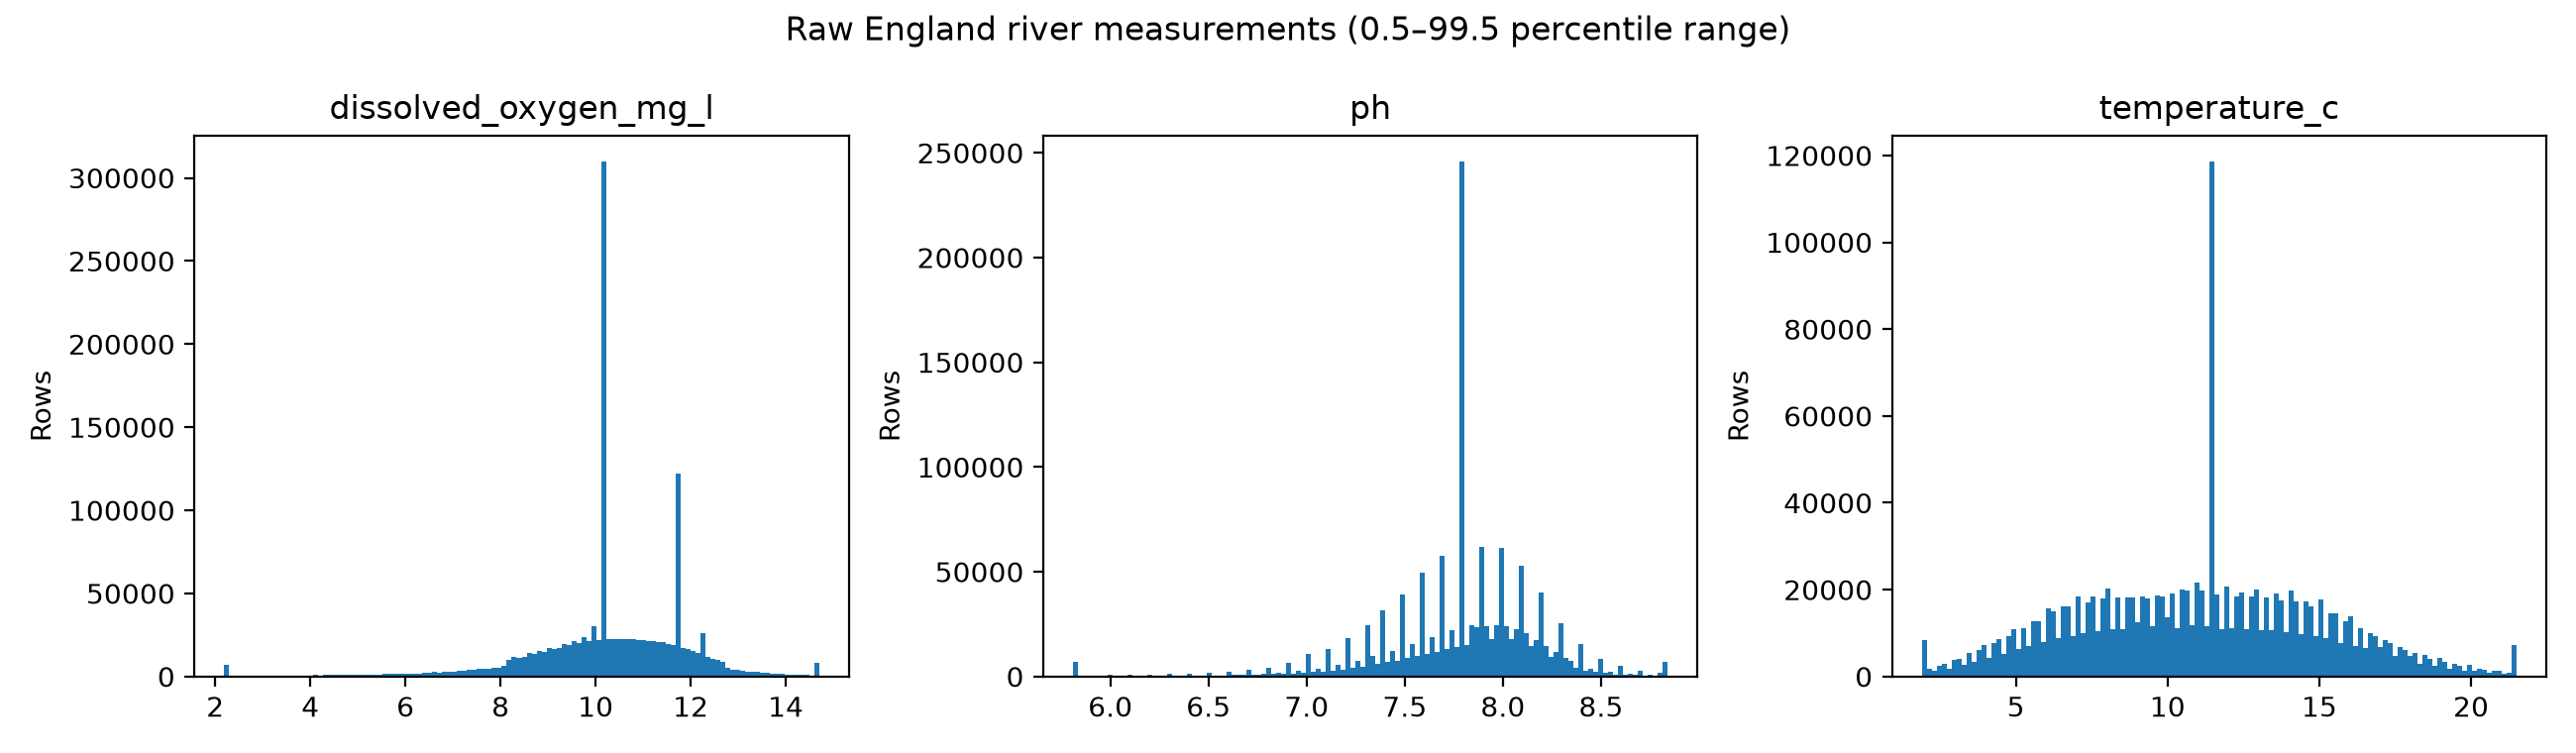
\includegraphics[width=0.85\textwidth]{../results/figures/eda_a4_raw_spikes.png}\caption{Raw England river data: the tall spikes are filler values.}\end{figure*}

\begin{figure}[!t]\centering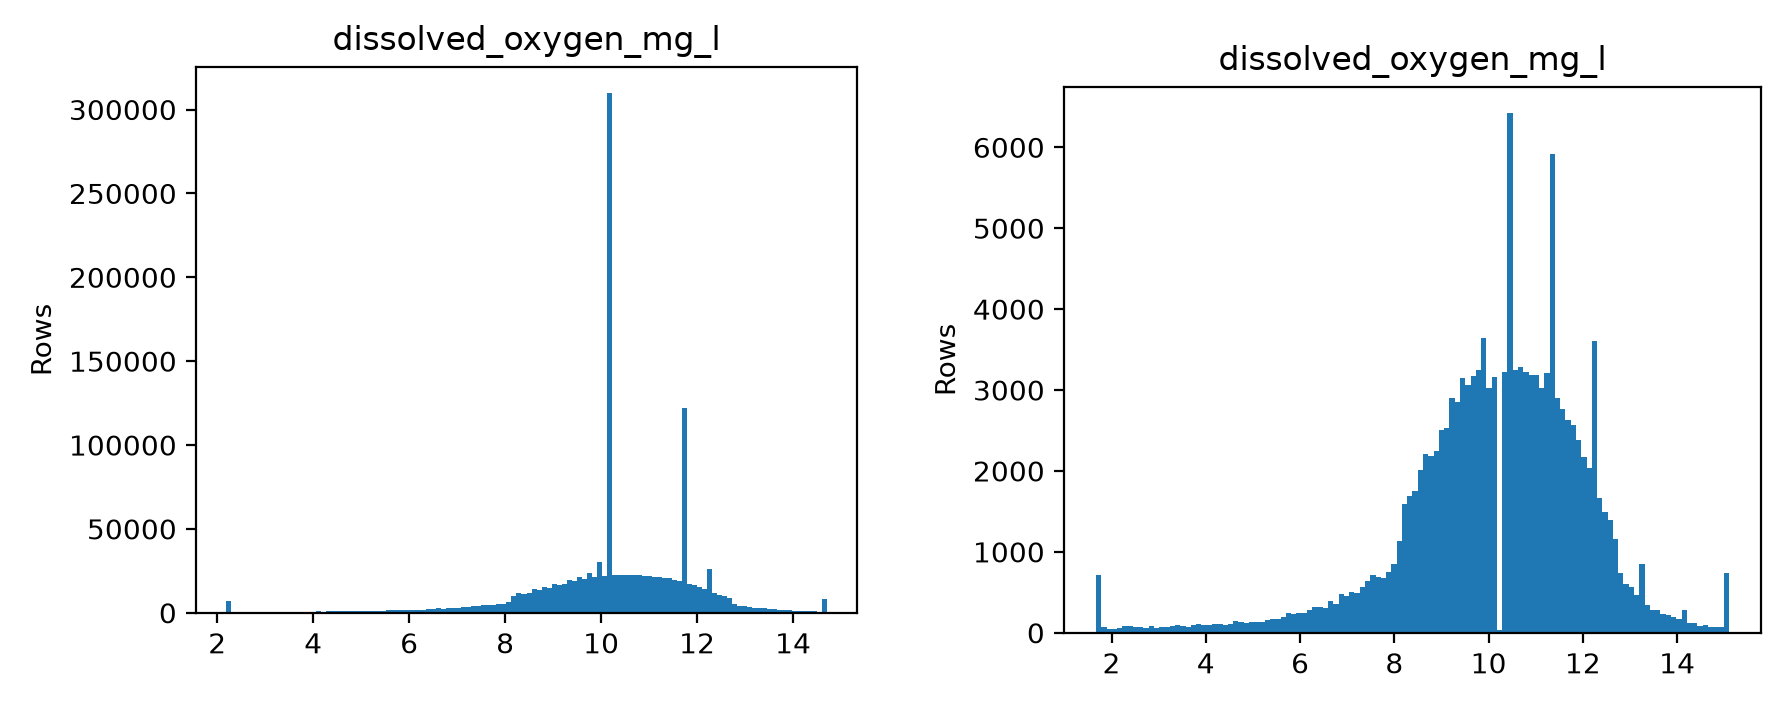
\includegraphics[width=\columnwidth]{../results/figures/eda_do_raw_vs_clean.png}\caption{England river dissolved oxygen, raw (left) and cleaned (right). The y-axes are different.}\end{figure}

We also set impossible values to missing instead of keeping them: for example 503 pH values outside 0 to 14, 222 temperatures outside -5 to 40 \textdegree{}C, and 3,564 BOD values above 150 mg/L. The cleaning also changed the country mix a lot. Most USA rows were filler, so the USA fell from 413,814 raw rows to 6,810 (14.9\% to 2.6\% of the data), Canada from 3,949 to 2,600, and England and Ireland now make up 69.3\% and 27.1\%.

\subsection{Missing values}
A missing value can also mean that the measurement was never taken at that place (Figure 3). BOD is missing in all USA rows, nitrogen in 76.5\% of Canadian rows and pH in 69.5\% of USA rows. Over all rows, BOD is missing in 51.7\%, ammonia in 29.4\% and nitrate in 23.8\%, while temperature (0.6\%) and pH (4.5\%) are almost always there. So the models fill gaps using the training data only, and also get a ``was missing'' flag.

\begin{figure}[!t]\centering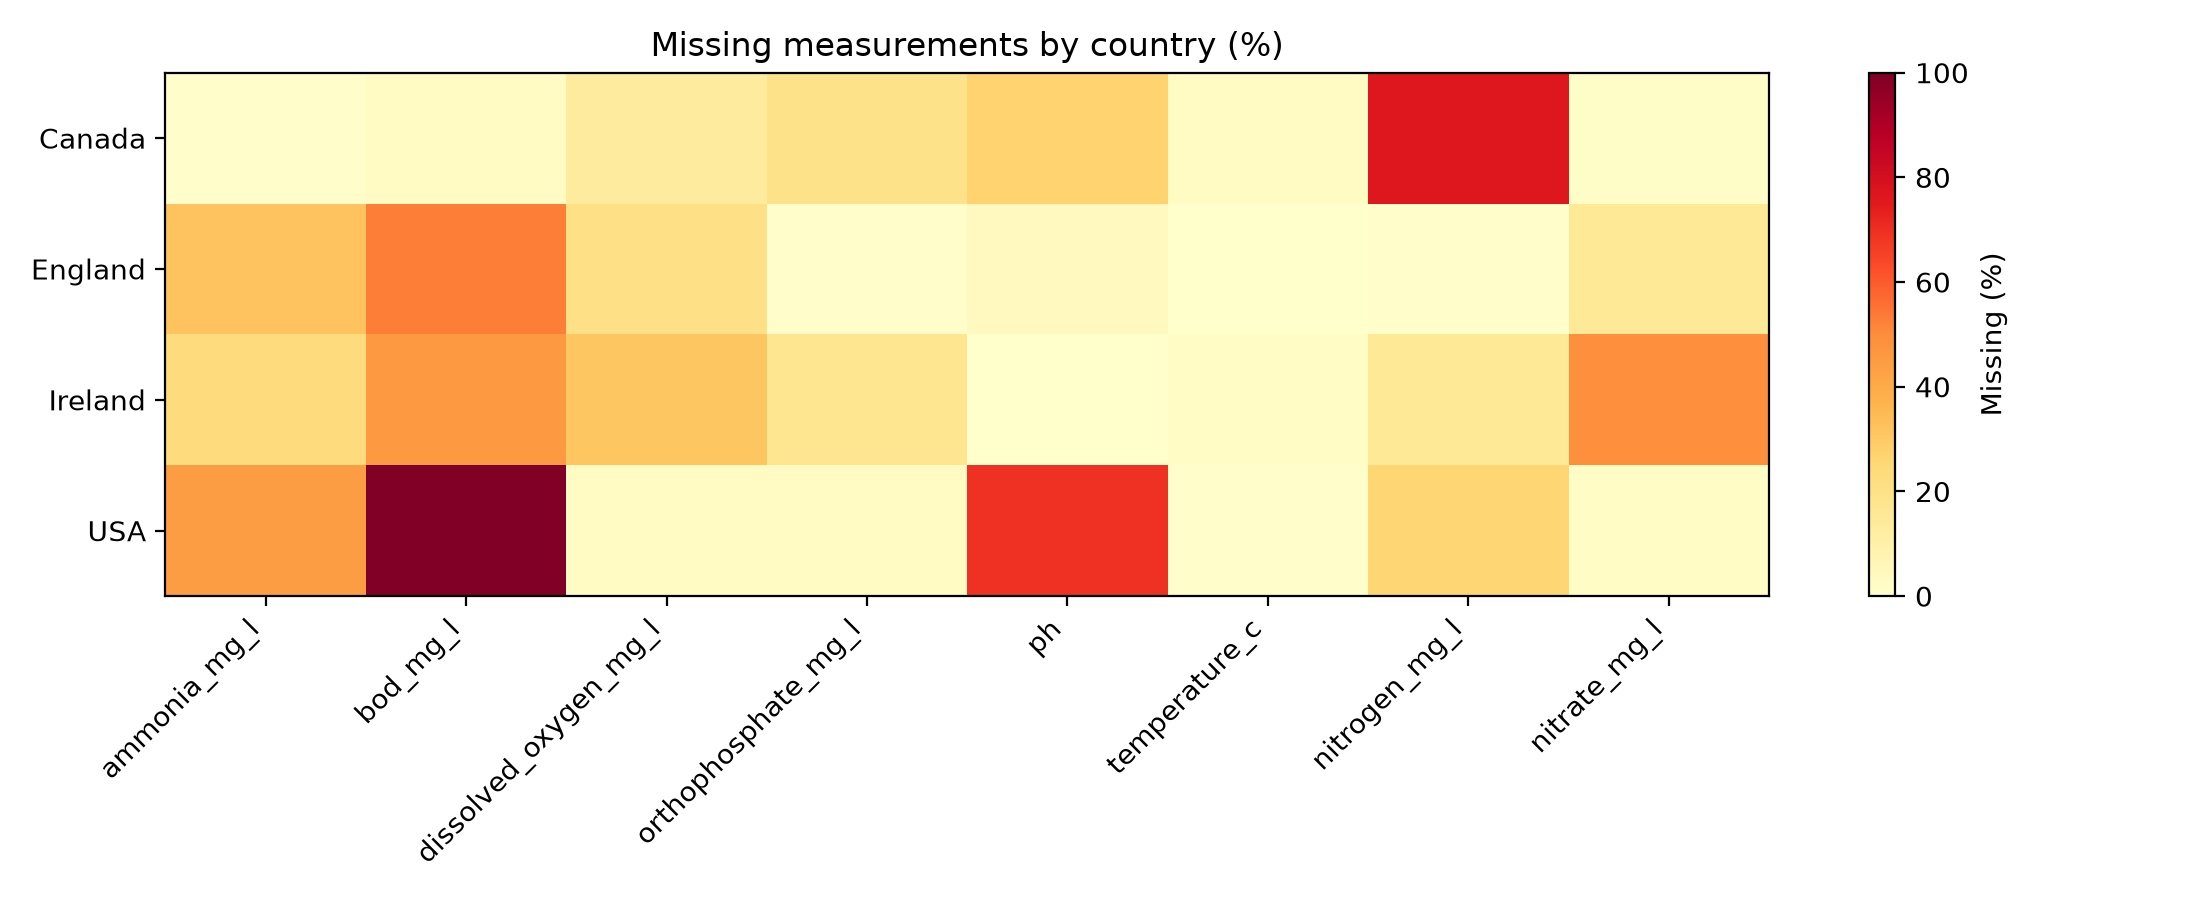
\includegraphics[width=\columnwidth]{../results/figures/eda_b3_missing_heatmap.png}\caption{Share of missing measurements for each country and parameter.}\end{figure}

\subsection{The target score}
43.7\% of all rows have a score of exactly 100 (Figure 4); Ireland has 81.6\% and England 28.9\%. By class, 43.7\% are Excellent, 39.9\% Good, 9.6\% Fair, 6.1\% Marginal and only 0.8\% Poor. There is very little data on bad water, so we also check the errors for each quality level.

\begin{figure*}[!t]\centering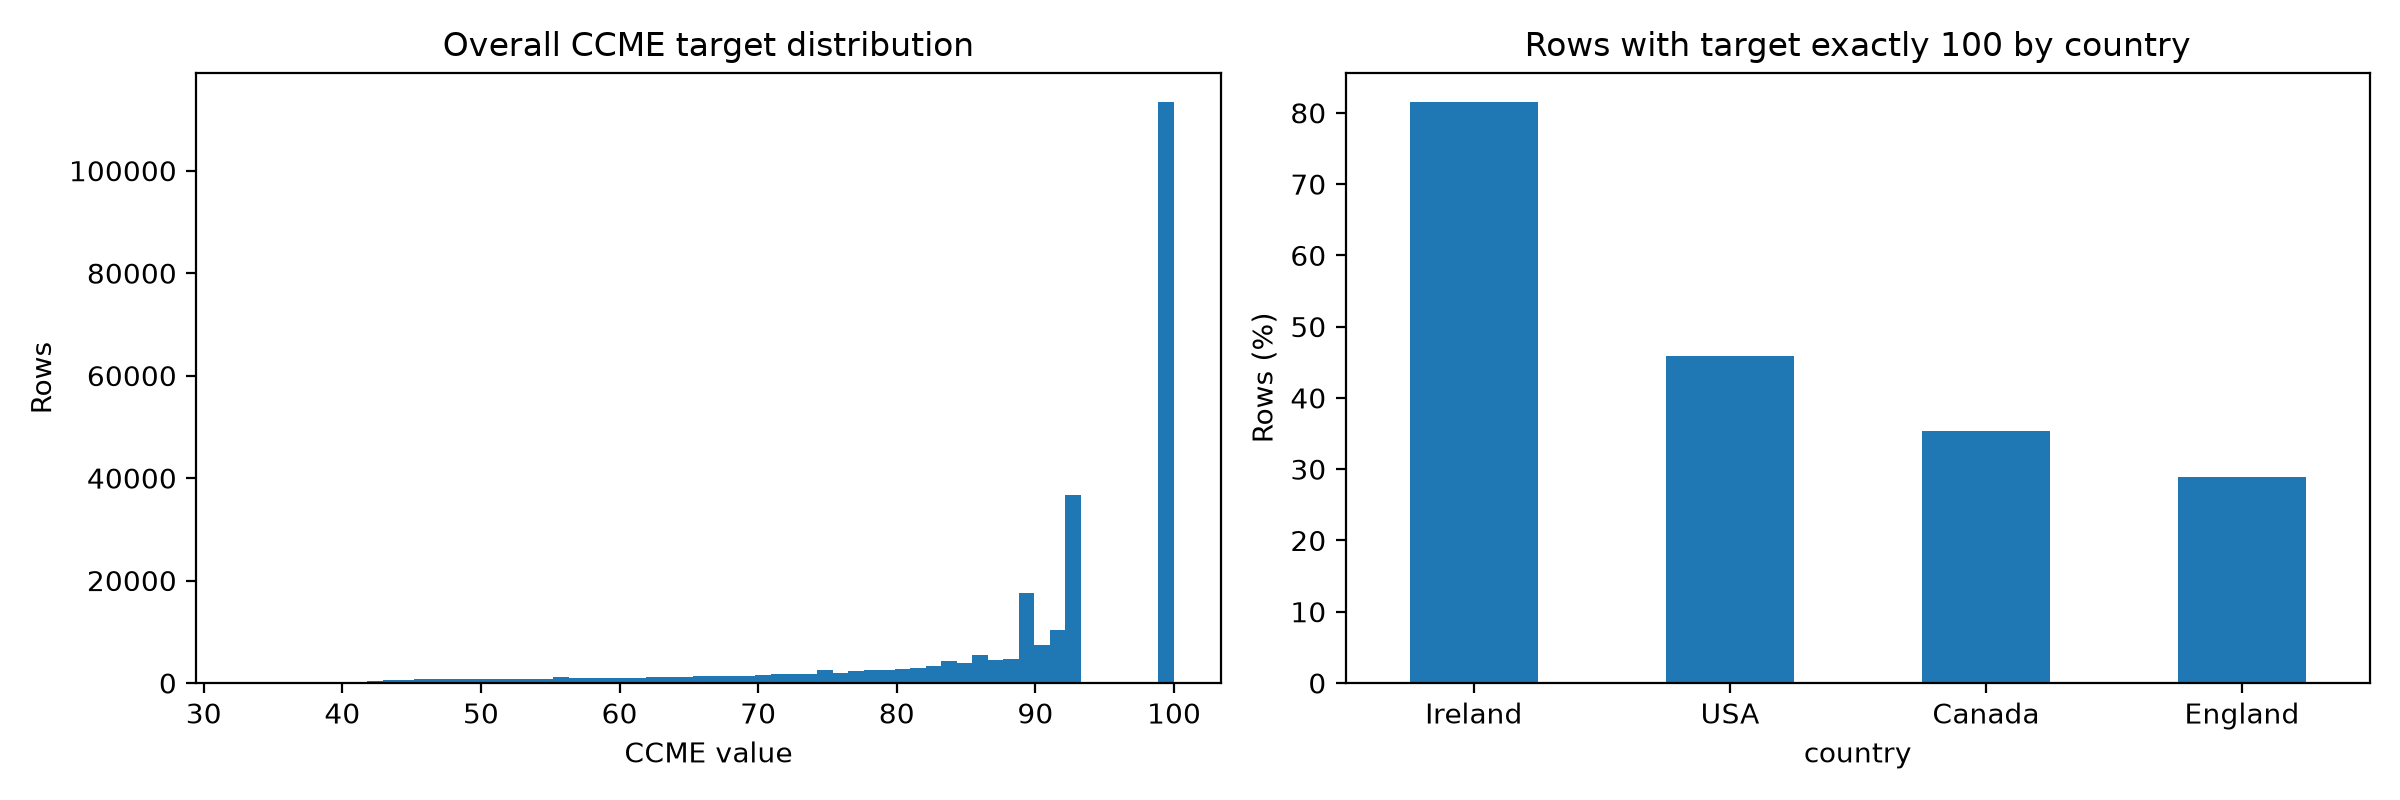
\includegraphics[width=0.85\textwidth]{../results/figures/eda_b4_target.png}\caption{Left: distribution of the CCME score. Right: share of rows with a score of exactly 100, by country.}\end{figure*}

\subsection{What drives the score}
We measured how strongly each measurement moves together with the score (Spearman correlation; negative means more of it gives a lower score, Figure 5). Orthophosphate is by far the strongest ($-$0.93), then ammonia ($-$0.54), nitrogen ($-$0.49), nitrate ($-$0.47) and BOD ($-$0.42). The sensor readings are weak alone: dissolved oxygen $-$0.10, pH $-$0.09, temperature $-$0.12. A model that sees the five strong ones can recompute the formula (Section~\ref{sec:leak}), so we hide them. A correlation shows that two things move together, not that one causes the other.

\begin{figure}[!t]\centering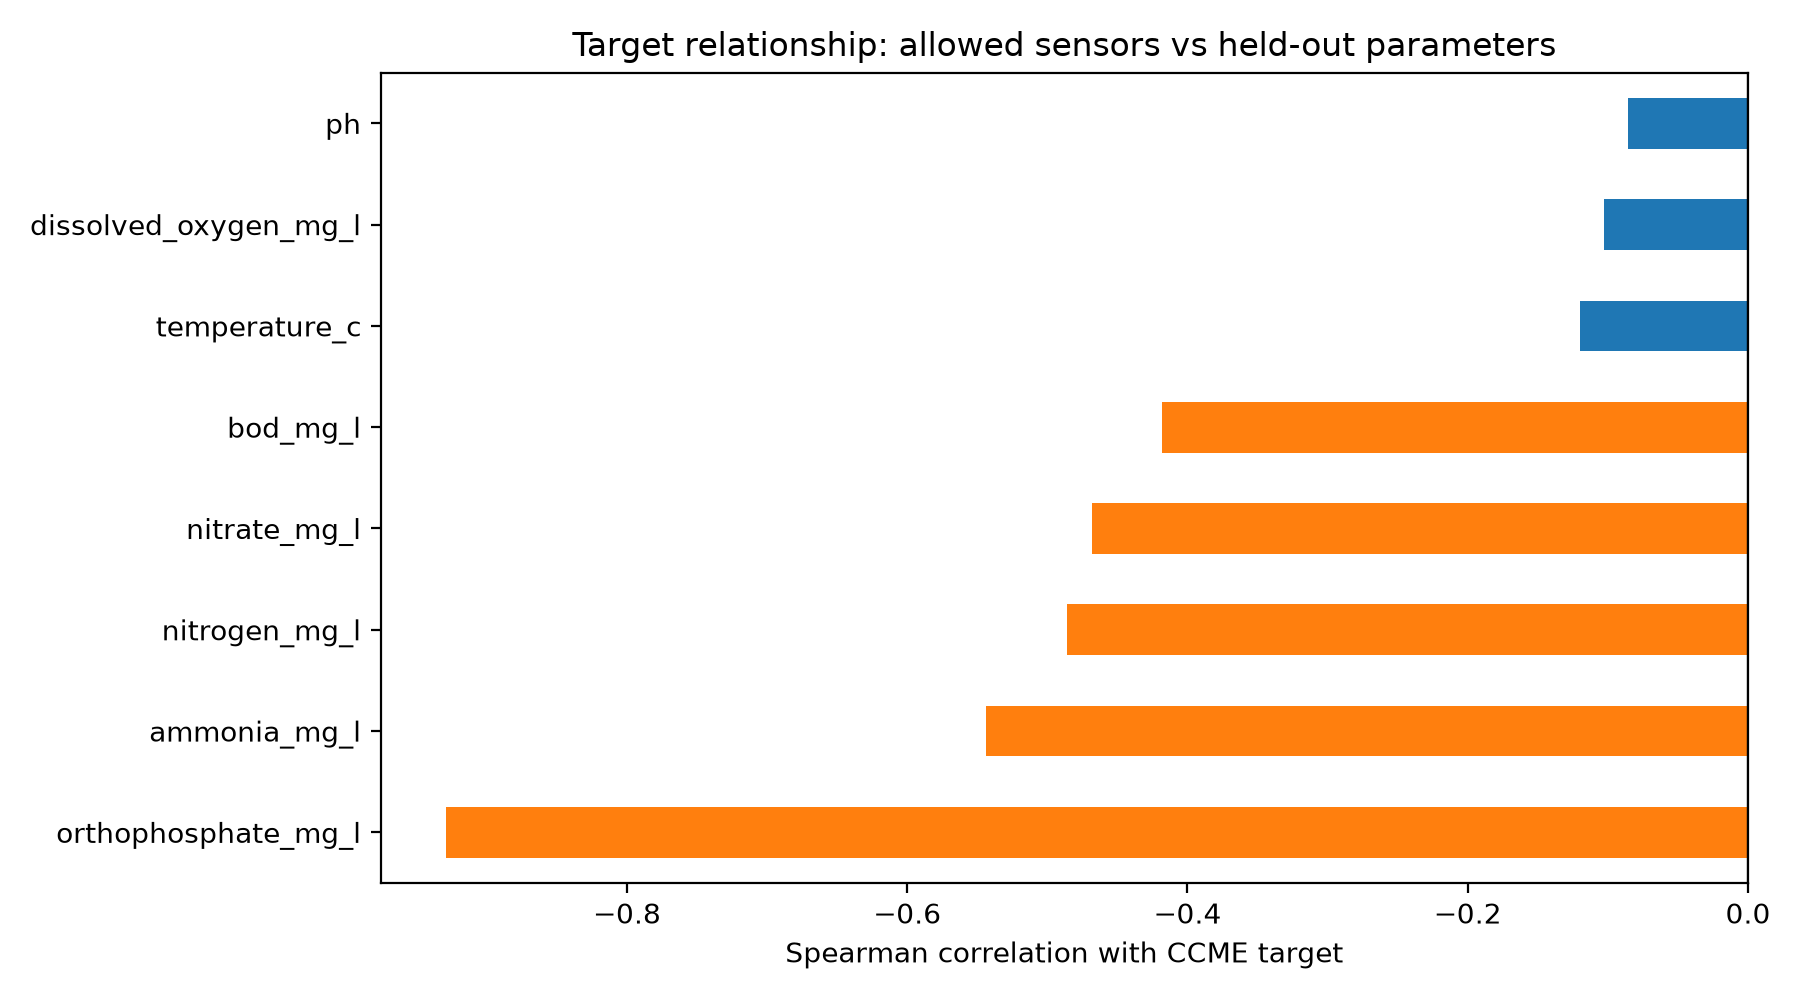
\includegraphics[width=\columnwidth]{../results/figures/eda_b5_corr.png}\caption{Correlation of each measurement with the score. Blue: allowed inputs. Orange: hidden from the model.}\end{figure}

\subsection{Stations, years and seasons}
Rows per year are fairly steady (about 7,000 to 14,000, with a dip in 2020, Figure 6). Stations are very uneven: the median station has 3 rows, 60\% have 5 or fewer, and one has 6,426. Rows of one station look alike, so a random split would put the same station in both training and test data. This is why our main split is by station.

\begin{figure*}[!t]\centering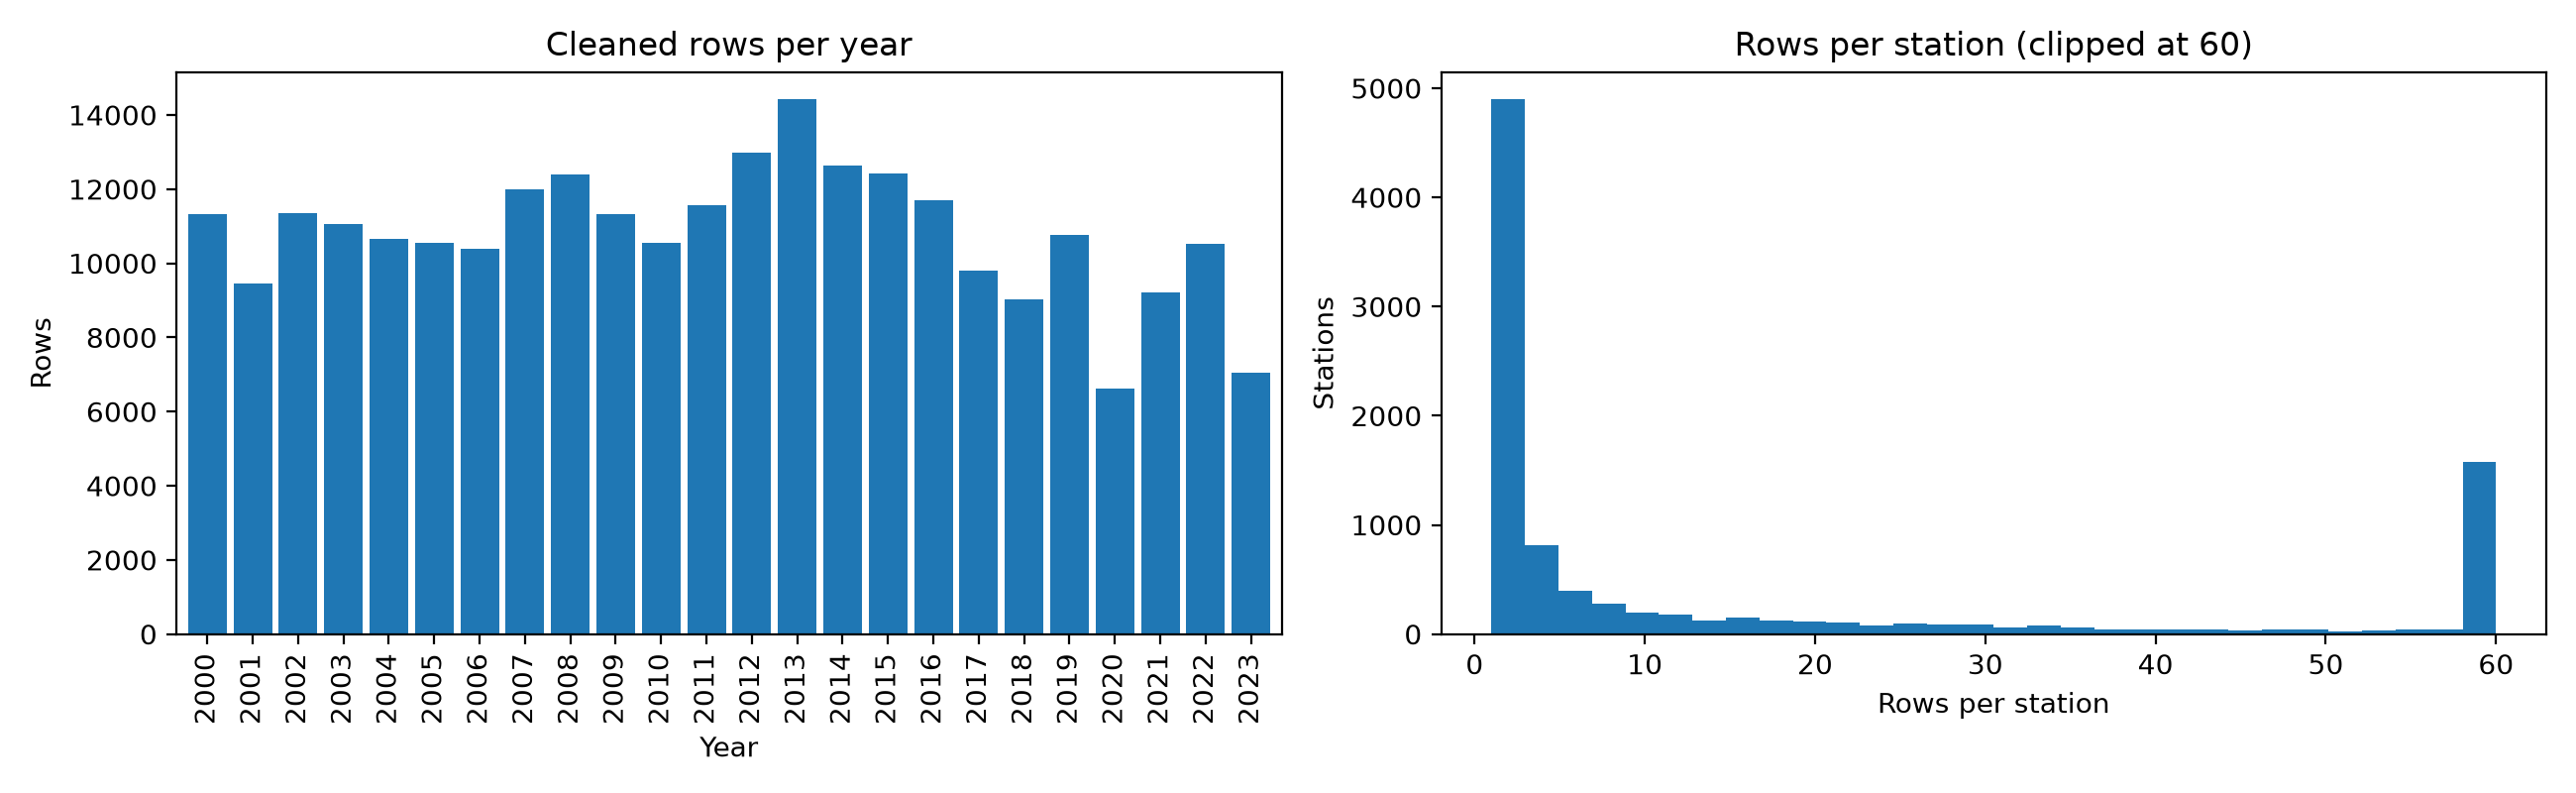
\includegraphics[width=0.85\textwidth]{../results/figures/eda_b6_year_site.png}\caption{Left: rows per year. Right: rows per station (stations with more than 60 rows are counted as 60).}\end{figure*}

The average score is lowest in July and August (88.5) and highest in February (91.8) (Figure 7), so we turn the month into a sine and a cosine, which puts December next to January.

\begin{figure*}[!t]\centering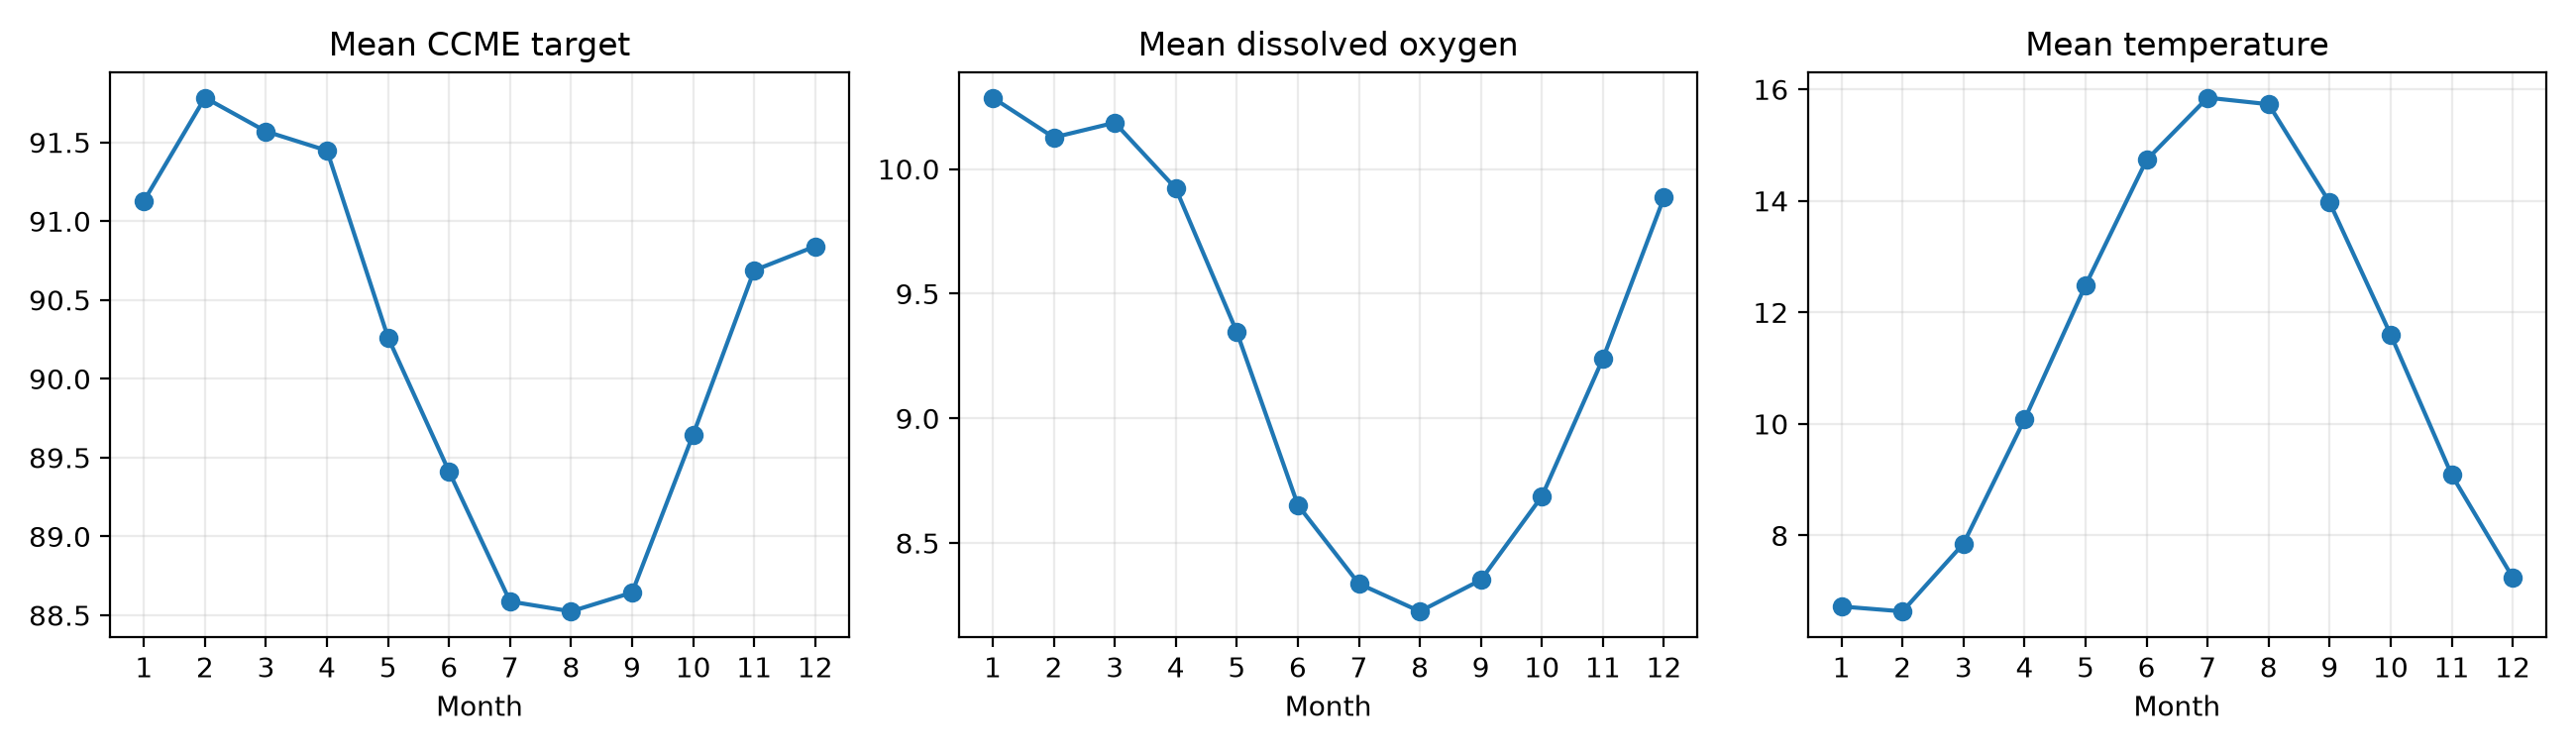
\includegraphics[width=0.85\textwidth]{../results/figures/eda_b8_season.png}\caption{Average score, dissolved oxygen and temperature by month.}\end{figure*}

\subsection{EDA on the cleaned data: raw vs cleaned}
After cleaning we repeated the EDA on the 259,774 remaining rows. The table compares the two versions. The raw file has no blanks, but only because gaps were filled with repeated numbers. After cleaning these are shown as missing, so the data are honest. The raw column shows the share of filler (cleaning log) and the cleaned column the share of missing values; they do not cover exactly the same rows, so the percentages are a guide.

\begin{table*}[!t]\caption{Raw data compared with cleaned data.}\centering
{\footnotesize\setlength{\tabcolsep}{3pt}\begin{tabular}{>{\raggedright\arraybackslash}p{0.26\linewidth}>{\raggedright\arraybackslash}p{0.17\linewidth}>{\raggedright\arraybackslash}p{0.17\linewidth}>{\raggedright\arraybackslash}p{0.24\linewidth}}\toprule
 & \textbf{Before (raw)} & \textbf{After (cleaned)} & \textbf{What we did better}\\\midrule
Rows & 2,781,980 & 259,774 & Only usable surface-water rows\\
Columns & 14 & 19 & Added year, month, split labels\\
Effluent, sewage, drainage rows & 635,532 & 0 & Removed non-river water\\
Country share: Eng / Irl / USA / Can (\%) & 76.5 / 8.5 / 14.9 / 0.1 & 69.3 / 27.1 / 2.6 / 1.0 & Less England-heavy, Canada visible\\
USA rows & 413,814 & 6,810 & Removed mostly filler-filled rows\\
Canada rows & 3,949 & 2,600 & Kept most real Canadian data\\
BOD & 58.9\% filler & 51.7\% missing & Filler marked as missing\\
Ammonia & 38.4\% filler & 29.4\% missing & Filler marked as missing\\
Dissolved oxygen & 35.0\% filler & 22.4\% missing & Spike gone, smooth shape\\
Nitrate & 31.2\% filler & 23.8\% missing & Filler marked as missing\\
pH & 16.5\% filler & 4.5\% missing & Almost always present\\
Temperature & 10.6\% filler & 0.6\% missing & Almost always present\\
\bottomrule\end{tabular}}
\end{table*}

In the raw England data (Figure 8, top) each measurement has a very tall thin spike, up to about 300,000 rows at a dissolved oxygen of exactly 10.2. After cleaning (bottom) the shape is a smooth hill with a tallest bar of about 6,000 rows. The two rows of plots use different y-axes.

\begin{figure*}[!t]\centering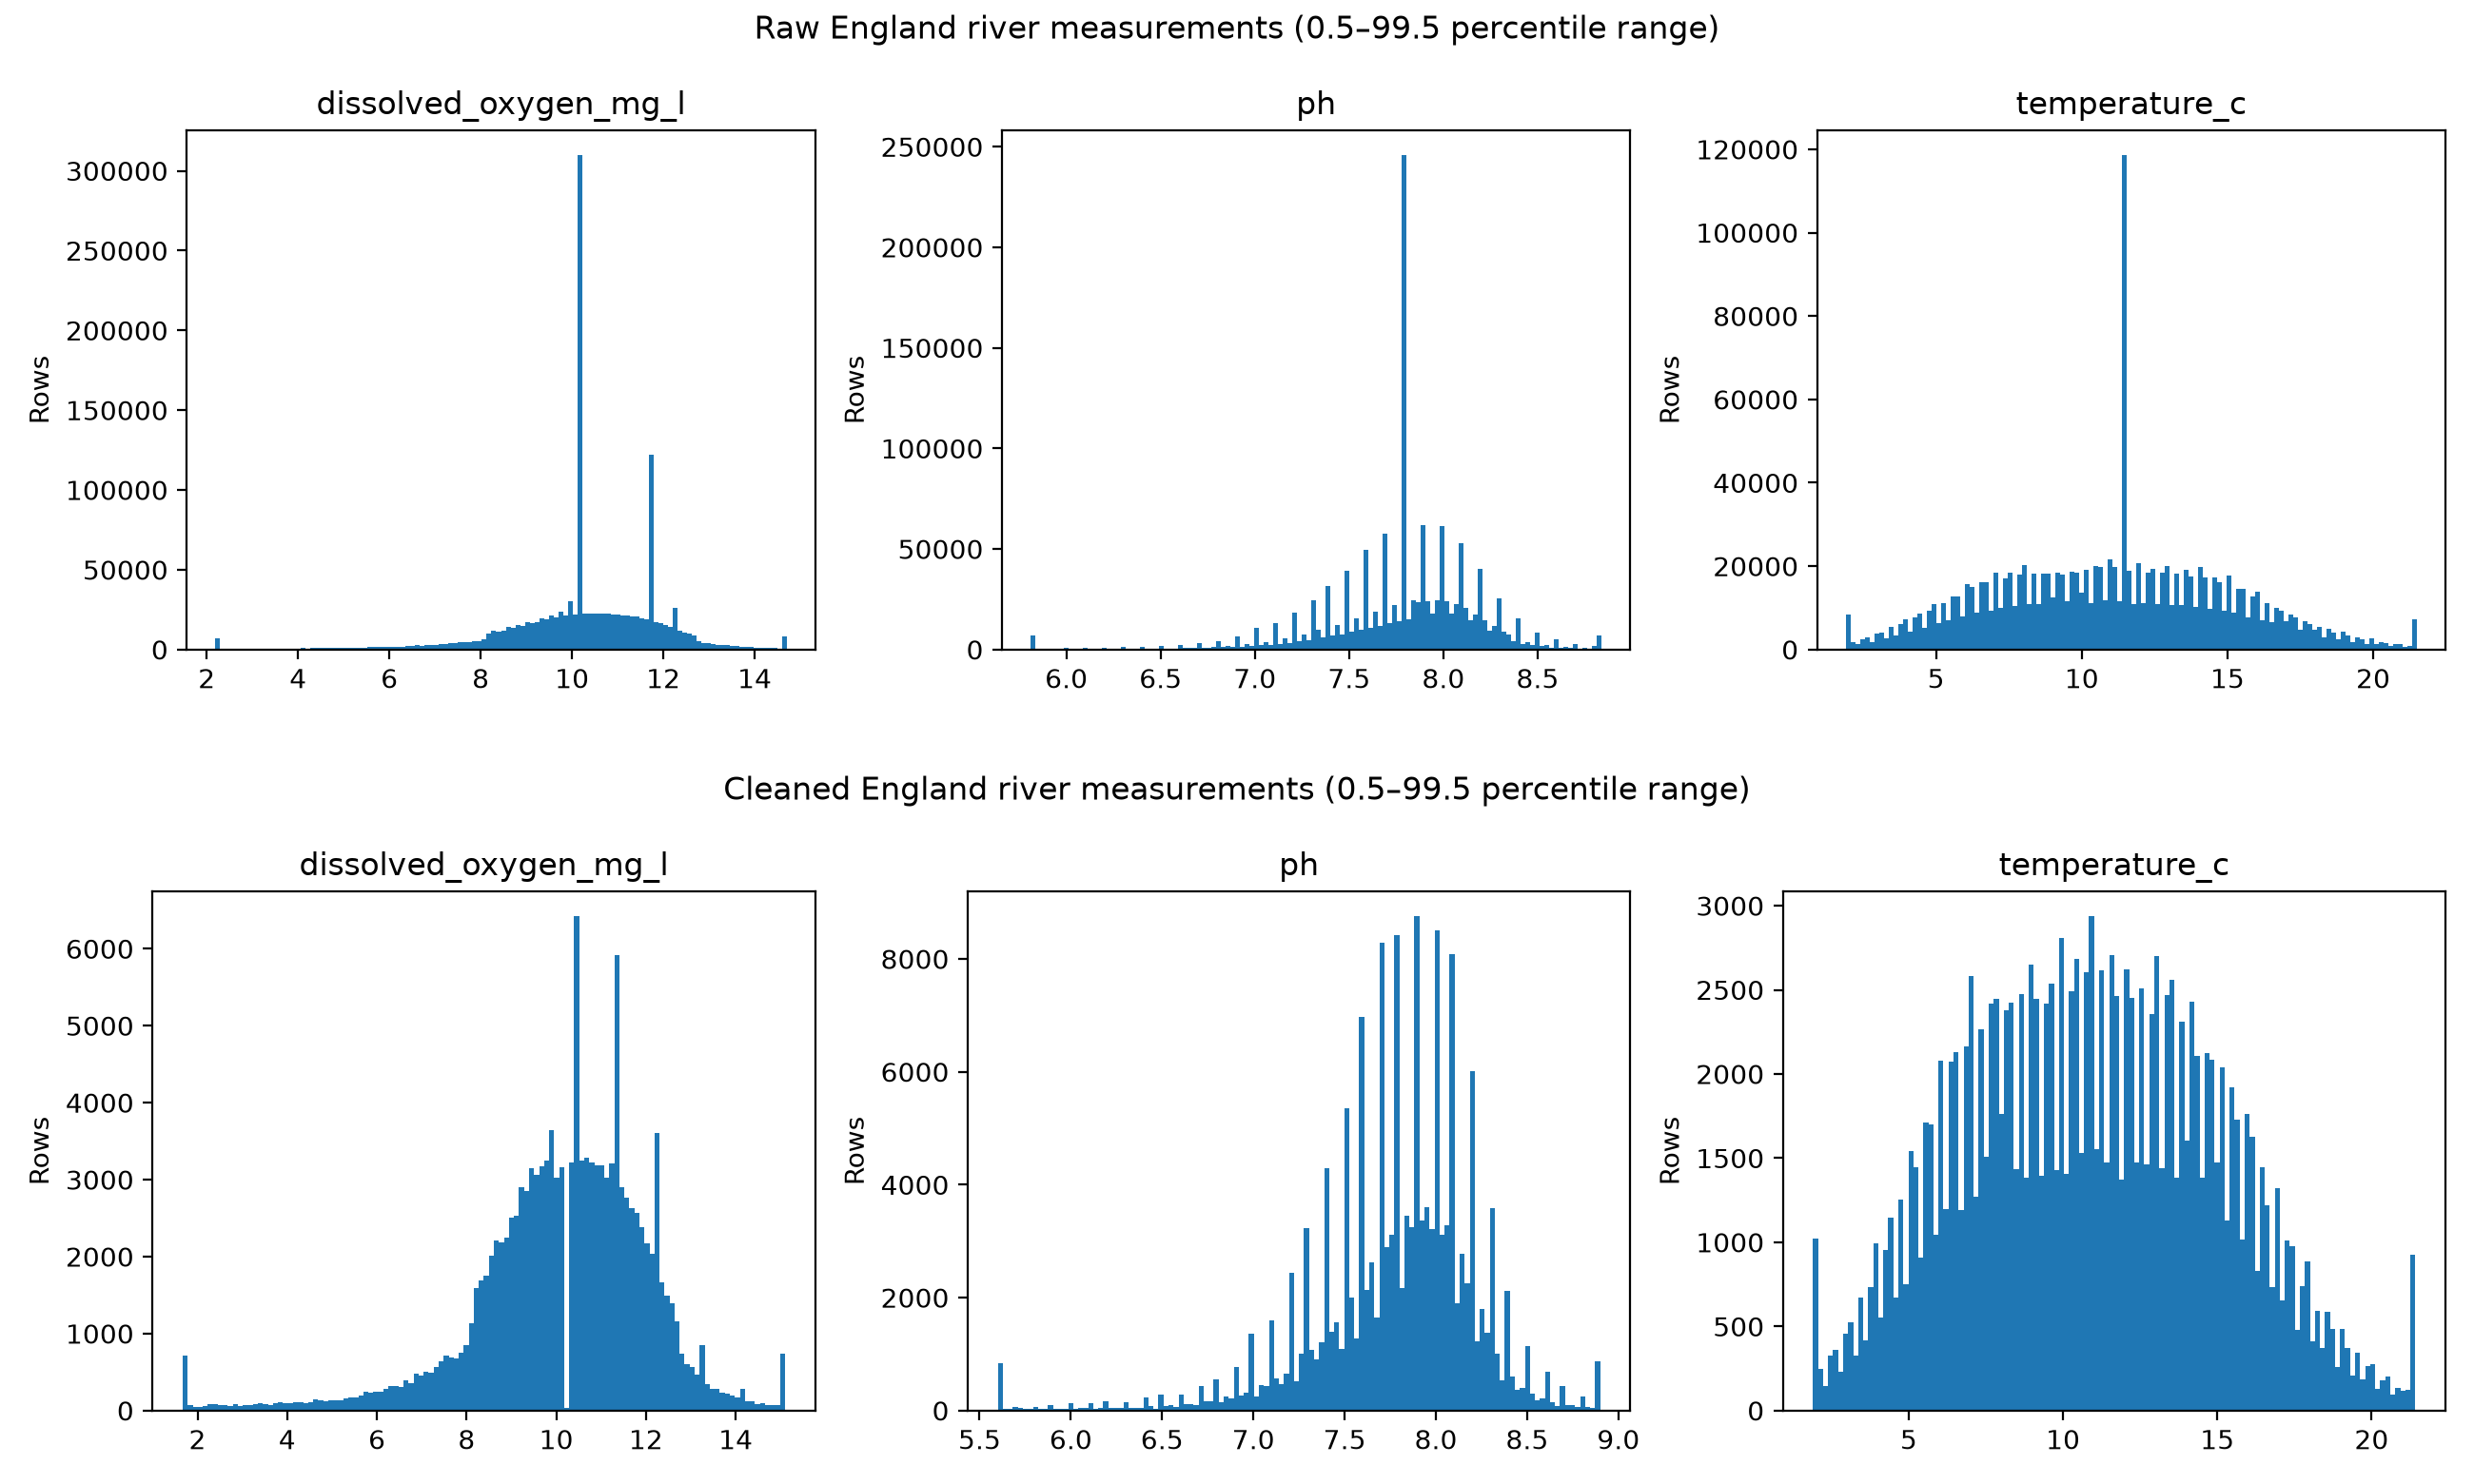
\includegraphics[width=0.85\textwidth]{../results/figures/eda_before_after_hists.png}\caption{England rivers, raw (top) and cleaned (bottom). The y-axes are different.}\end{figure*}

In short, the cleaned data are smaller but cleaner: no sewage rows, no pre-2000 records, no duplicates, no filler spikes, and a better balance between countries.


\section{Method}
\subsection{Avoiding data leakage}\label{sec:leak}
The index is calculated from eight measurements: ammonia, BOD, dissolved oxygen, orthophosphate, pH, temperature, nitrogen and nitrate. We trained XGBoost on different input sets and scored it on the validation data. With all eight the score was R$^2$ = 0.991, and with our first proposed set 0.982, so the model had simply learned the formula. We therefore removed ammonia, BOD, orthophosphate, nitrogen and nitrate. Dissolved oxygen, pH and temperature are also part of the index, but each alone explains very little (R$^2$ at most 0.04).

\begin{table}[!t]\caption{Validation $R^2$ of XGBoost for different input sets.}\centering
{\footnotesize\setlength{\tabcolsep}{3pt}\begin{tabular}{>{\raggedright\arraybackslash}p{0.62\linewidth}r}\toprule
\textbf{Inputs given to XGBoost} & \textbf{Validation R$^2$}\\\midrule
All eight measurements & 0.991\\
First proposal (pH, temperature, ammonia, orthophosphate, nitrogen, type) & 0.982\\
Dissolved oxygen, pH, temperature only & 0.127\\
+ water type, country, month & 0.268\\
+ extra features and station history (chosen) & 0.343\\
Baseline (always the average) & $-$0.005\\
\bottomrule\end{tabular}}
\end{table}

\subsection{Features and preprocessing}
The models use 14 inputs: dissolved oxygen, pH, temperature, the month (as a sine and a cosine), oxygen saturation, dissolved oxygen $\times$ temperature, the station's average past dissolved oxygen, pH and temperature, the number of earlier samples at the station, days since the previous sample, water body type and country. Past averages only use earlier dates of the same station, so nothing from the future is used. Missing values are filled with the training median (plus a ``was missing'' flag), categories are one-hot encoded, and values are scaled for Ridge only. All of this is learned from the training data only.

\subsection{Train, validation and test split}
Our main split is \textbf{by station}: all rows of a station go to one part only, with 70\% of rows for training, 10\% for validation and 20\% for testing (181,747 / 26,054 / 51,973 rows from 6,583 / 1,136 / 2,221 stations). The test then shows how a model does at a place it has never seen; a random split would let it remember stations. Our second split is \textbf{by year}: training up to 2015, validation 2016--2017, test 2018 onwards. Settings are chosen on the validation data only, and the test data are used once at the end.

\subsection{Models and tuning}
The baseline always predicts the training average. Ridge Regression is a straight-line model with a penalty that keeps the numbers small. Random Forest averages many deep decision trees. XGBoost builds trees one after another, each fixing the mistakes of the earlier ones. We tuned each model on the validation data with a small grid, changing one setting at a time: Ridge $\alpha$ 0.001 to 1000; Random Forest depth 6--16 and minimum leaf size 2--20 (300 trees); XGBoost depth 4--10, learning rate 0.03--0.1 and 300 or 600 trees.

The settings with the lowest validation RMSE were chosen: Ridge $\alpha$ = 0.001; Random Forest depth 16 and minimum leaf size 5; XGBoost depth 8, learning rate 0.03, 300 trees, row sampling 0.8, feature sampling 0.8 and L2 weight 1.0. The random seed was 42.

\subsection{Metrics and confidence intervals}
\[\mathrm{MAE}=\frac{1}{n}\sum_i |y_i-\hat y_i|\]
\[\mathrm{RMSE}=\sqrt{\frac{1}{n}\sum_i (y_i-\hat y_i)^2}\]
\[R^2=1-\frac{\sum_i (y_i-\hat y_i)^2}{\sum_i (y_i-\bar y)^2}\]
MAE is the average size of the error, and RMSE gives more weight to big errors; lower is better for both. R$^2$ shows how much better the model is than always guessing the average: 1 is perfect, 0 is no better. A test set is only one sample of stations, so we repeated the evaluation 2,000 times on stations drawn again at random (keeping all rows of a station together) and used the middle 95\% of results as the confidence interval. To compare two models, we used the same re-drawn stations for both and looked at the difference in their errors.


\section{Results}
\subsection{Validation results}
On the validation data XGBoost was best (MAE 7.729, RMSE 11.205, R$^2$ = 0.348), just ahead of Random Forest (7.773, 11.247, 0.343). Ridge reached R$^2$ = 0.219 and the baseline $-$0.005. On the training data Random Forest scored R$^2$ = 0.558 and XGBoost 0.461, so Random Forest overfits more.

\subsection{Test on unseen stations}
\begin{table}[!t]\caption{Test results on unseen stations (95\% bootstrap intervals).}\centering
{\footnotesize\setlength{\tabcolsep}{3pt}\begin{tabular}{>{\raggedright\arraybackslash}p{0.33\linewidth}rrrr}\toprule
\textbf{Model} & \textbf{MAE} & \textbf{RMSE} & \textbf{R$^2$} & \textbf{95\% CI for R$^2$}\\\midrule
Baseline (average) & 9.570 & 13.159 & $-$0.001 & [$-$0.009, 0.000]\\
Ridge & 8.329 & 11.733 & 0.205 & [0.174, 0.233]\\
Random Forest & 7.598 & 11.179 & 0.278 & [0.230, 0.324]\\
\textbf{XGBoost} & \textbf{7.543} & \textbf{11.058} & \textbf{0.293} & [0.246, 0.340]\\
\bottomrule\end{tabular}}
\end{table}

XGBoost is the best model. Its confidence interval overlaps with Random Forest, but on the same re-drawn stations its RMSE was lower by 0.121 (95\% interval $-$0.186 to $-$0.059), so it is better in a consistent way, but only slightly. Both tree models are clearly better than Ridge (RMSE 0.674 lower for XGBoost) and the baseline (2.101 lower). Still, R$^2$ below 0.30 means most of the variation in the score is not explained.

The test R$^2$ is lower than the validation R$^2$ (0.293 against 0.348), partly because we picked settings that looked best on validation, and probably because the test stations are harder. We did not separate these two reasons.

\begin{figure}[!t]\centering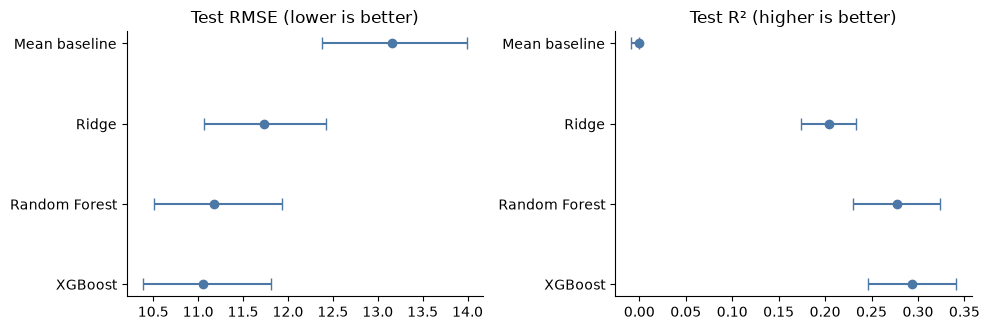
\includegraphics[width=\columnwidth]{../results/figures/eval_ci.png}\caption{Confidence intervals of the test scores.}\end{figure}

\subsection{Test on later years}
The models were trained again on the year split with the same settings. These numbers should not be mixed with the station test, because the test data are different (the negative baseline R$^2$ shows that scores changed after 2015). The order of the models stays the same.

\begin{table}[!t]\caption{Test results on later years (year split).}\centering
{\footnotesize\setlength{\tabcolsep}{3pt}\begin{tabular}{>{\raggedright\arraybackslash}p{0.40\linewidth}rrr}\toprule
\textbf{Model (2018 onwards)} & \textbf{MAE} & \textbf{RMSE} & \textbf{R$^2$}\\\midrule
Baseline (average) & 9.101 & 10.693 & $-$0.338\\
Ridge & 6.738 & 8.786 & 0.097\\
Random Forest & 5.596 & 8.310 & 0.192\\
\textbf{XGBoost} & \textbf{5.449} & \textbf{8.047} & \textbf{0.243}\\
\bottomrule\end{tabular}}
\end{table}

\subsection{Where do the models go wrong?}
The overall score hides big differences between countries. England is 70\% of the test rows, and the model helps least there (MAE only 6\% below the baseline). Ireland shows the biggest improvement, but 82\% of its samples are exactly 100, so its R$^2$ is close to zero. The USA and Canada have few rows, so their results are less reliable.

\begin{table}[!t]\caption{XGBoost test performance by country.}\centering
{\footnotesize\setlength{\tabcolsep}{3pt}\begin{tabular}{>{\raggedright\arraybackslash}p{0.28\linewidth}rrrr}\toprule
\textbf{Country} & \textbf{Rows} & \textbf{MAE} & \textbf{Baseline MAE} & \textbf{R$^2$}\\\midrule
England & 36,396 & 9.25 & 9.86 & 0.194\\
Ireland & 14,443 & 3.30 & 8.91 & 0.026\\
USA & 580 & 5.88 & 9.35 & 0.156\\
Canada & 554 & 7.63 & 8.15 & 0.080\\
\bottomrule\end{tabular}}
\end{table}

\begin{figure}[!t]\centering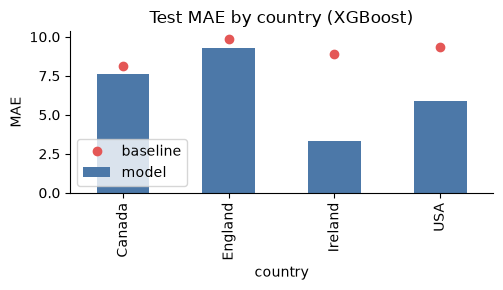
\includegraphics[width=\columnwidth]{../results/figures/eval_by_country.png}\caption{XGBoost test performance by country.}\end{figure}

The error also depends on the true water quality. When the true score is below 60, the model guesses about 31 points too high on average, and for perfect water (100) about 5.5 points too low, so guesses are pulled towards the middle. The five main measurements are hidden, so the model cannot tell when water is really bad, and 44\% of samples are exactly 100, so a ``fairly good'' guess is usually safe. Several of the hardest stations are near sewage works or industrial discharges.

\begin{table}[!t]\caption{XGBoost error by true water quality level.}\centering
{\footnotesize\setlength{\tabcolsep}{3pt}\begin{tabular}{>{\raggedright\arraybackslash}p{0.34\linewidth}rrr}\toprule
\textbf{True score} & \textbf{Rows} & \textbf{MAE} & \textbf{Mean error}\\\midrule
below 60 & 2,719 & 30.98 & +30.98\\
60 to 80 & 6,032 & 12.52 & +12.15\\
80 to 95 & 20,502 & 5.19 & $-$1.90\\
100 & 22,720 & 5.54 & $-$5.52\\
\bottomrule\end{tabular}}
\end{table}

\begin{figure}[!t]\centering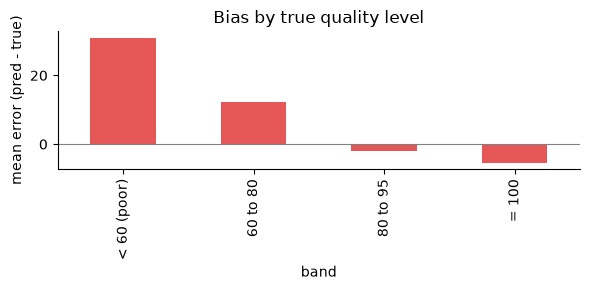
\includegraphics[width=\columnwidth]{../results/figures/eval_bias_by_band.png}\caption{Average error of XGBoost by true water quality level.}\end{figure}

\begin{figure}[!t]\centering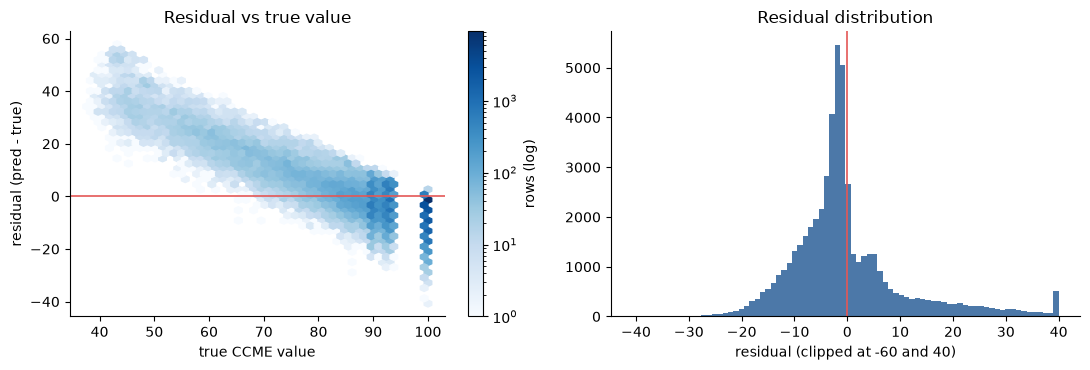
\includegraphics[width=\columnwidth]{../results/figures/eval_residuals.png}\caption{Errors of the test predictions.}\end{figure}

\subsection{Which inputs matter?}
We trained XGBoost again with some inputs removed. With all inputs R$^2$ was 0.348; without country 0.274, without the station history 0.271, and without both 0.162. SHAP (3,000 test rows) agrees: country is the most important input (average effect 4.75 points), then the station's past dissolved oxygen (1.40), temperature (1.32) and past pH (1.19). So much of the score comes from knowing the country and station, which may not work in a new region.

\begin{figure}[!t]\centering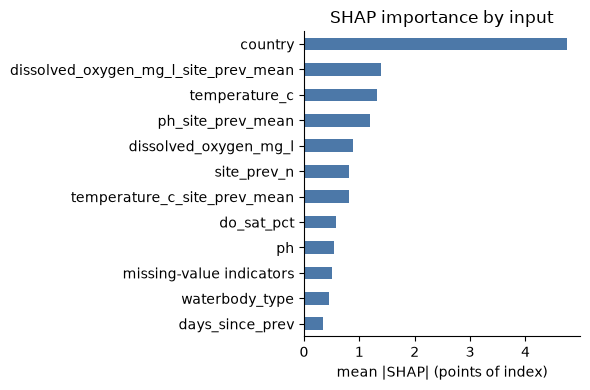
\includegraphics[width=\columnwidth]{../results/figures/eval_shap_grouped.png}\caption{Importance of each input for XGBoost (SHAP).}\end{figure}


\section{Discussion}
The tree models beat the baseline and Ridge even with the reduced inputs. XGBoost is best on both tests and Random Forest is close; XGBoost's lead is real but small. R$^2$ is lower on later years than on new stations because the data are different, not because one split is better. Many samples sit at 100, so we report MAE, RMSE and R$^2$ together with results by country and quality level. The biggest weakness is that polluted water is predicted as better than it is, which is the more harmful mistake in real monitoring.


\section{Limitations and future work}
The model cannot replace laboratory tests. Countries and monitoring practices differ, and the filled-in values in the source data may affect the score. The test R$^2$ is moderate, as expected with the five main measurements hidden. We tuned on one validation split without cross-validation, so validation scores are somewhat optimistic, and the best Random Forest depth and XGBoost learning rate were at the edge of our grid. England has most of the data, while the USA and Canada have very little.

In Phase 2 we plan to train a small neural network (MLP) on the same inputs and splits, compare it fairly without touching the test set while choosing the model, and check stations from regions with little data.


\section{Conclusion}
We compared a baseline, Ridge Regression, Random Forest and XGBoost for predicting the CCME index without the measurements it is calculated from. On unseen stations XGBoost gave MAE 7.543, RMSE 11.058 and R$^2$ = 0.293, slightly but consistently better than Random Forest; on later years MAE 5.449, RMSE 8.047 and R$^2$ = 0.243. Tree models are a good start, but they over-estimate poor water and rely much on country and station history. The next step is a fair comparison with a neural network.

\bibliographystyle{IEEEtran}\bibliography{references}
\end{document}
